\documentclass[10pt,conference]{IEEEtran}
\usepackage{xspace}
\usepackage{url}
\usepackage[pdftex]{graphicx}
\usepackage{wrapfig}

\DeclareGraphicsExtensions{.pdf,.png}

\begin{document}

\newcommand{\durationTotal}{6626\xspace}
\newcommand{\durationCorresponding}{2\xspace}
\newcommand{\durationWorking}{10\xspace}
\newcommand{\durationVM}{10\xspace}
\newcommand{\durationVagrant}{15\xspace}
\newcommand{\durationWorkingOnWorkable}{10\xspace}
\newcommand{\durationWorkingOnUnWorkable}{10\xspace}
\newcommand{\emailsSent}{3\xspace}
\newcommand{\emailsRecieved}{2\xspace}
\newcommand{\durationAuthorResponse}{15\xspace}
\newcommand{\durationAuthorResponseCountHigh}{20\xspace}
\newcommand{\emailsHelpful}{82\%\xspace}
\newcommand{\emailsFriendly}{85\%\xspace}
\newcommand{\emailsIntimidating}{4\%\xspace}
\newcommand{\emailsAnnoyed}{10\%\xspace}
\newcommand{\emailsPercentSent}{92\%\xspace}
\newcommand{\contactOSSed}{2\xspace}
\newcommand{\contactFixLink}{3\xspace}
\newcommand{\contactHosted}{4\xspace}
\newcommand{\contactFixBug}{8\xspace}
\newcommand{\contactFixDepl}{2\xspace}
\newcommand{\papersWithLinks}{62\%\xspace}
\newcommand{\papersWithLinksDead}{7\%\xspace}
\newcommand{\papersWithLinksRevived}{44\%\xspace}
\newcommand{\obtainPaper}{42\%\xspace}
\newcommand{\obtainGoogle}{19\%\xspace}
\newcommand{\obtainEmail}{20\%\xspace}
\newcommand{\obtainNot}{20\%\xspace}
\newcommand{\onlineGitHub}{25\%\xspace}
\newcommand{\onlineSourceforge}{3\%\xspace}
\newcommand{\onlineGcode}{2\%\xspace}
\newcommand{\onlinePersonalSite}{28\%\xspace}
\newcommand{\onlineNotAvail}{39\%\xspace}
\newcommand{\onlineCodeplex}{2\%\xspace}
\newcommand{\onlineBitbucket}{3\%\xspace}
\newcommand{\onlineJustGcode}{2\xspace}
\newcommand{\working}{60\%\xspace}
\newcommand{\workingNum}{86\xspace}
\newcommand{\totalToolsTried}{143\xspace}
\newcommand{\unworkPay}{2\xspace}
\newcommand{\unworkInternal}{9\xspace}
\newcommand{\unworkNoResponseToAsk}{13\xspace}
\newcommand{\unworkTooLate}{3\xspace}
\newcommand{\unworkCouldntWorkIt}{19\xspace}
\newcommand{\serviceRunning}{8\xspace}
\newcommand{\serviceRunningLater}{2\xspace}
\newcommand{\serviceRunningNever}{4\xspace}
\newcommand{\redistPermissionArtifact}{43\xspace}
\newcommand{\redistPermissionEmail}{31\xspace}
\newcommand{\licenseMIT}{7\xspace}
\newcommand{\licenseGPL}{5\xspace}
\newcommand{\licenseApache}{7\xspace}
\newcommand{\licenseGPLThree}{4\xspace}
\newcommand{\licenseBSD}{6\xspace}
\newcommand{\licenseLGPL}{2\xspace}
\newcommand{\licenseMPL}{2\xspace}
\newcommand{\licenseEPL}{14\xspace}
\newcommand{\depWindows}{22\xspace}
\newcommand{\depVS}{6\xspace}
\newcommand{\permissionToRedistribute}{49\xspace}


\newcommand{\projectLikeThis}{45\%\xspace}
\newcommand{\projectLikeOther}{26\%\xspace}
\newcommand{\projectDontCare}{30\%\xspace}

%TODO how are you dealing with the non-representative sample of tools from really early -- 2011?

\title{Reviving \workingNum of \totalToolsTried of Tools from ICSE and FSE}

\author{\IEEEauthorblockN{Emerson Murphy-Hill, Shabbir Abdul, Varun Aettapu, Sumeet Agarwal, Sindhu Anangur Vairavel,\\Rishi Avinash Anne, Haris Mahmood Ansari, Ankit Bhandari, Bhanu Anand, Aditya Vinayak Bhise,\\Saikrishna Teja Bobba, Vineela Boddula, Venkata Krishna Sailesh Bommisetti, Dwayne Christian (Chris) Brown, Jr.,\\Peter Morgan Chen, Yi Chun ({Yi-Chun}) Chen, Nikhil Chinthapallee, Karan Singh Dagar,\\Joseph Decker, Pankti Rakeshkumar Desai, Jayant Dhawan, Yihuan Dong, Sarah Elizabeth Elder, Shrenuj Gunvant Gandhi,\\Jennifer Michelle Green, Mohammed Hasibul Hassan, Satish Inampudi, Pragyan Paramita Jena,\\Bhargav Rahul ({Bhargav}) Jhaveri, Apoorv Vijay Joshi, Nikhil Josyabhatla, Sujith Katakam, Juzer Husainy Khambaty,\\Aneesh Arvind Kher, Craig Kimpel, Siddhartha Kollipara, Asish Prabhakar Kottala, Abishek Kumar,\\Harini Reddy Kumbum, Nitish Pradeep Limaye, Apoorv Mahajan, Sai Sindhur Malleni, Sudha Manchukonda,\\Kavit Maral Mehta, Justin Alan Middleton,Ramakant Moka, Eesha Gopalakrishna Mulky, Gauri Naik,\\Shraddha Anil Naik, Yashwanth Nallabothu, Yogesh Nandakumar, Kairav Sai Padarthy, Pulkesh Kumar Yadav Pannalal,\\Sattwik Pati, Kahan Prabhu, Shashank Goud Pulimamidi, Gargi Sandeep Rajadhyaksha, Priyadarshini Rajagopal,\\Venkatesh Sambandamoorthy, Mohan Sammeta, Shaown Sarker, Anshita Sayal, Vrushti Kamleshkumar Shah,\\Esha Sharma, Saurav Shekhar, Sarthak Prabhakar Shetty, Manish Ramashankar Singh,\\Ankush Kumar Singh, Vinay Kumar Suryadevara, Sumit Kumar Tomer, Akriti Tripathi, Jennifer Tsan,\\Vivekananda Vakkalanka, Alexander Valkovsky, Rishi Kumar Vardhineni, Manav Verma}
\IEEEauthorblockA{Department of Computer Science\\
North Carolina State University\\
Raleigh, North Carolina, USA\\
emerson@csc.ncsu.edu}\{sabdul,vaettap,sagarwa6,sanangu,raanne,hmansari,abhanda3,bhanua,avbhise,sbobba3,vboddul,\\vbommis,dcbrow10,pmchen,ychen74,nchinth,kdagar,jdecker,prdesai2,jdhawan2,ydong2,seelder,sgandhi4,jmgree17,mhhassan,\\sinampu,ppjena,bjhaver,avjoshi,njosyab,skataka,jhkhamba,aakher,ckimpal,skollip,akottal,akumar21,hkumbum,nplimaye,\\amahaja3,smallen3,smanchu,kmmehta,jamiddl2,rmoka,egmulky,gnaik2,sanaik2,ynallab,ynandak,kspadart,ppannal,spati2,\\kprabhu,spulima,gsrajadh,prajago4,vsamban,msammet,ssarker,asayal,vkshah,esharma2,sshekha3,spshetty,mrsingh,asingh21,\\vksuryad,sktomer,atripat4,jtsan,vvakkal,avalkov,rkvardhi,mverma4\}@ncsu.edu}



\maketitle
\begin{abstract}
Many innovative software engineering tools appear at the field's premier venues, the 
International Software Engineering Conference (ICSE) and the 
Foundations of Software Engineering (FSE).
But what happens to these tools after they are presented?
In this paper, we describe a course project where we spent 
thousands of person hours
trying to obtain, download, use, and repackage \totalToolsTried
tools from ICSE and FSE's tool demonstration tracks from
2011 through 2014.
Our results enumerate the practical and accidental reasons that
software engineering tools fail to work over time,
and provide practical implications for creating lasting 
research tools.
%TODO do you deliver on this?
\end{abstract}

\begin{IEEEkeywords}
software engineering tools; replication
\end{IEEEkeywords}

\section{Introduction}

Software engineering research seeks to better understand how software is built
and constructed. While such understanding in isolation can be insightful,
ultimately the bulk of such research aims to impact practice. To do so,
researchers can recommend new software engineering practices, design educational
techniques and materials, and create tools.

Creating new tools is arguably the most common way that software engineering
researchers attempt to influence practice. % evidence? would be good to see what
% the primary contributions are of a recent ICSE or FSE?
Broadly speaking, tools are software that can help design and build software.
Examples include a tool that helps mobile application developers choose which
devices to target~\cite{prada}, a tool that checks the use of locks in
multithreaded programs~\cite{ernst}, and a tool that creates code from natural
language text~\cite{desai}.

While papers describe tools in software engineering venues,
there are several reasons why software engineering researchers 
should make the tools themselves available.
First, the full details of how the tool works, both in terms of its internals
and from an end-user perspective, may not be clear from the paper.
Second, making the tools available can help practitioners try and adopt
the tools in their work.
Third, it helps the advancement of the field by allowing others to build on 
existing tools, rather than rebuilding them from scratch.
Finally, it helps facilitate replicability by enabling future researchers
to perform studies with the original tools.
In this paper, we use the term replicability~\cite{vim2004international}
to refer to ``an independent group [obtaining] the same result using 
the author's own artifacts''~\cite{acmArtifactPolicy}.
Although artifacts in replications also commonly includes data,
in this paper we focus on software.

Despite the benefits of making tools available, in this paper
we catalog the practical difficulties in doing so.
We describe a study that examined the tools presented at the 
premier venues for software engineering research over the 
past several years.
As part of a graduate university course on software engineering, 
we spent \durationTotal hours trying to obtain, download, use
and repackage tools from the International Conference
on Software Engineering (ICSE) and the Symposium on the Foundations
of Software Engineering (FSE).
In doing so, we make the following three main 
contributions in this paper:

\begin{itemize}
  \item A study that evaluates the difficulty in getting \totalToolsTried tools 
  		working across a variety of software engineering research.
  \item A synergistic course project for graduate software engineering students 
		that gives students meaningful educational value \emph{and}
		%TODO is this fair, given students didn't think they learned a lot?
		provides the research community value.
  \item \permissionToRedistribute existing tools repackaged in automatically-built virtual machines
  		to make it easier for others to use these tools.
\end{itemize}

\section{Related Work}

% Other fields:
% - Data science (doing better - http://zenodo.org)
% - MPC journal requires code submission (tarball)
% - In general, Math not doing a lot with code sub submissions
% - Security, should be able to do VM, but don't (but see Will's paper)
% - HPC doesn't (and maybe can't)
% - RTC is starting to do it, but maybe shouldn't
% Constant worry is protecting IP in security and HPC

\subsection{Replicability in Science Policy}

%TODO more theory here
%See Tim's paper he sent

Our study is one specific foray into the topic of replicability
in science, an area whose importance researchers and the public 
increasingly cite.
Ince and colleagues ``argue that, with some exceptions, anything less 
than the release of source programs is intolerable for 
results that depend on computation''~\cite{ince2012case}.

Both in science generally and in computer science specifically,
the urgency of increasing replicability has increased sharply.
In a 2016 survey of 1500 scientists across disciplines, the journal
Nature reported that 70\% of researchers had attempted
and failed to replicate others' experiments~\cite{baker20161}.
A 2015 study in the journal Science 
attempted to replicate 100 psychology experiments,
finding that a ``large portion of replications produced weaker evidence for the original findings''~\cite{open2015estimating}.

In computer science, the Association for Computing Machinery has
recently formed the ``Task Force on Data, Software, and Reproducibility in Publication''
and the ``Replication Taskforce.''
The goals of these taskforces are to 
``promote practices that lead to better replicability''~\cite{acmDataTaskforce} and 
``develop proposals on how ACM can bring current replication and 
verification practices in line with the rest of the scientific 
community''~\cite{acmRepTaskforce}.
While both task forces are actively working as of this writing, 
in 2016 they released a policy that recommends certification of
replicability and reproducibility~\cite{acmArtifactPolicy}.
But because few replication studies exist in computer science,
the motivation for this policy is based on studies
``primarily in the biomedical field.''
Our study provides data to inform such evolving policies.

\subsection{Replicability Studies in Computer Science}

Some computer science sub-disciplines have attempted to replicate
research involving software.
Kova{\v{c}}evi{\'c} evaluated 15 image processing papers,
finding that algorithm descriptions were
generally adequate, but that none of the papers provided
implementations~\cite{kovacevic2007encourage}.
Later, Vanderwalle and Kova{\v{c}}evi{\'c} repeated that study on 134 
image processing papers and found that 84\% provided implementation details
and 9\% provided code~\cite{vandewalle2009reproducible}. 
Our study differs in that we went beyond finding out whether code was available;
we ran and repackaged that code.

Callberg and Proebsting's recent replicability study~\cite{collberg2016repeatability,proebsting2015repeatability},
published after we had completed our study, is most similar to ours. 
In it, the authors examined the systems described in 
601 papers from 13 systems conferences from 2011 to 2013
(including, relevant to our paper, OOPSLA and PLDI 2012).
Of those papers:

\begin{itemize}   
\item in 85 cases, the authors provided code in the article; 
\item in 54 cases, code could be found via web search;
\item in 87 cases, the authors provided code upon request;
\item in 146 cases, authors refused to provide the code; and
\item in 30 cases, authors did not respond to email.
\end{itemize}

\noindent
Furthermore, Callberg and Proebsting's team tried to get the tools to build, finding
that:

\begin{itemize} 
\item in 130 cases, the code was built in 30 minutes or less;
\item in 64 cases, the code was built in more than 60 minutes;
\item in 23 cases, the code's original authors assured the team that the code could be
			built; and
\item in 9 cases, the code could not be built.
\end{itemize}

\noindent
Apart from studying tool demonstrations from software engineering venues
rather than technical papers from systems venues,
our study primarily complements Callberg and Proebsting's study in two
ways.
First, we used a stricter standard of acceptance; rather than just building
the tool, we verified that the tool ran as described in the original paper.
Second, in addition to validating that a tool worked, we attempted to 
repackage the tools as a contribution to the community, so that other
researchers would not have to duplicate our efforts. 

Other papers in software engineering have also explored 
replicability of tools.
Klein and colleagues selected 9 papers from ICFP 2009 to
re-implement as formal models in their domain-specific language;
they found mistakes in all 9 papers~\cite{klein2012run}.
Mende attempted to replicate prior results using two 
existing defect predictors, finding that even
``with access to the original data sets, replicating
previous studies may not lead to the exact same results''~\cite{mende2010replication}.
More recently, Shepperd and colleagues' replicated 42 studies 
using defect predictors, finding that the research group 
performing the analysis has a strong effect on performance~\cite{shepperd}.
Likewise, Tantithamthavorn and colleagues' replication of this meta-study
confirmed these results, but explained the problem as arising from 
research groups reusing datasets and metrics~\cite{tantithamthavorn}.
Our study complements these papers in that we evaluate a wider
variety of software engineering tools.

\subsection{Artifact Evaluation Committees}

Researchers in programming languages, and to a lesser extent
software engineering, have recently implemented steps
to increase reproducibility by forming
\emph{artifact evaluation committees} (AECs).
AECs run in parallel with program committees,
and aim to review research artifacts, including tools.
At the top software engineering conferences,
AECs have been run at the main technical track of 
Foundations of Software Engineering 2011 and 2013 through 2015.
Accepted research papers are encouraged, but not required, to 
submit artifacts to AECs.
Accepted artifacts may or may not be archived by 
the authors after the conference.

At least 10 past instantiations of AECs have reported data about 
their outcomes, which Collberg and colleagues summarize~\cite{proebsting2015repeatability}.
They find that typically about half of authors of accepted papers
choose to submit artifacts, and that acceptance rates for those
artifacts vary substantially.

The results of AECs and our study have 
similar goals and technical approaches.
Both aim to evaluate the artifact's 
consistency with the paper,
completeness,
documentation,
and ease of use~\cite{evaluate}.
From a technical standpoint, AECs generally  
encourage packaging of artifacts in virtual machines.

However, AECs and our study are different in several
ways.
AECs sometimes evaluate non-tools, such as data analysis scripts; 
our study evaluates only software engineering tools.
AECs report only data from artifacts that authors choose to submit;
we report data about all tools published at a 
conference's tool demonstration track.
AECs evaluate artifacts packaged by the authors themselves;
we report on tools that we package ourselves as outsiders.
AECs aim to evaluate artifacts during publication;
our study aims to evaluate tools years after publication.
AECs do not require the public distribution of artifacts;
distribution of artifacts is one of our primary goals.

Regardless of the similarities and differences,
our study motivates the need for AECs by demonstrating
the situations in which tools ``disappear'' years
after publication.
At the same time, our study highlights some significant
challenges to AECs by demonstrating the several
fundamental reasons tools cannot be archived. 


\section{Research Questions}

In this paper, we will simply say \emph{tool}
to refer to software engineering tools presented at
the International Conference on Software Engineering
or Foundations of Software Engineering in their
tool demonstration tracks.
We use the term \emph{researchers} to refer to 
the creators of the tool described in the paper. 

In this paper we answer the following research questions:

\begin{itemize}
  
\item\textbf{RQ1.} \textit{How much effort is required to get tools to work?}
If these costs are high (say, requiring more than a few hours), 
then researchers need extra support and incentives for 
making their tools trialable.

\item\textbf{RQ2.} \textit{What are the barriers to get tools to work?}
Enumerating these barriers explains what kind of additional
support researchers need for making their tools trialable.

\item\textbf{RQ3.} \textit{What are the barriers to get tools to work in virtual machines?}
Virtual machines are preferred for sharing tools with AECs~\cite{guidelines}; 
these barriers imply what additional support is
necessary, and what the limitations are, of packaging and 
distributing tools in this way.

\item\textbf{RQ4.} \textit{Can tool packaging be implemented as a course project?}
If our course is feasible to do again, 
students could package future tools on behalf of researchers.
\end{itemize}

\section{Course Description}

We conducted the study described in this paper as 
part of a graduate software engineering course
in the Computer Science department at 
North Carolina State University.
The department has about 200 PhD students and 450
MS students in its graduate program.
While graduate students are not required to
take the course, it is one of seven core systems
courses, from which students must take one or two courses.
The department does have a specialty MS degree
track in software 
engineering~\cite{mstrack},
which does require this course.

Course content covers software engineering processes,
software architecture, design patterns, software security,
verification and validation, estimation, project management,
requirements, certification, and formal 
methods~\cite{syllabus}.
Apart from the course content, involving lectures and
a final exam, the other
major component of the course is the project.
Next, we describe the project for this course 
in prior offerings of the course (Section~\ref{sec:priorProj})
and in the offering described in this paper (Section~\ref{sec:thisProj}).

\subsection{Prior Course Project and Criticism}\label{sec:priorProj}

In prior offerings of the course,
students were essentially given two project offerings.
In one version, students could create
a software engineering tool, such as a plugin for Eclipse.
In the other version, students chose several existing,
similar software engineering tools, and applied them
to open source software, then reflected 
on what they learned about the tools and the 
projects.
Most students opted for the second version.
In both cases, students were required to write up their results.
This project is similar to a course project
assigned by David Notkin at the 
University of Washington~\cite{gradSEUW}.

After offering this project to students for 
several years, the instructor recognized several
problems in the way he had executed it:

\begin{itemize}  
  \item The course did not have enough time to teach students
  		technical writing skills, and thus final papers were 
  		of poor quality, on average. Moreover, while technical
  		communication is a course objective, other types of
  		communication would likely be more valuable to most
  		students, who are non-thesis and industry-focused.   		 
  \item Students had limited exposure to state-of-the-art
  		tools; the tools they chose to study were typically
  		quite basic.
  \item Students appeared to rarely gain technical skills 
  		during the project.  
  \item Most students were not doing \emph{novel} work; each semester,
  		different students wrote similar reports on similar tools,
  		which had no value beyond their educational value. 
\end{itemize}

While the last point may seem odd -- why would a course project need
value beyond its educational value? -- it's not unusual for 
some software engineering courses to have an added value,
such as contributing to open source projects~\cite{pedroni2007open,meneely2008rose}.
In the case of the present course, the instructor thought 
that such system development would not be useful to most students
in the course, who typically come in with 1 to 2 years of 
industrial software engineering experience. 

\subsection{New Course Project}\label{sec:thisProj}

In the Fall of 2015, the instructor changed the course project
to alleviate the problems described in the last subsection.
In short, student teams were assigned tools described in a 
prior research paper at ICSE or FSE, the premier 
venues for software engineering research.
Students were required to obtain the tools, get them running,
and redistribute them.

The instructor chose tool demonstration papers, rather than
full technical papers, for practical reasons.
Full technical papers may not present a tool; for 
instance, a purely qualitative study that reports on 
empirical findings may have no software to go along with it.
In contrast, tool demo papers almost certainly have a working
tool when the paper is presented at a conference. 

There were several learning goals of the course project:

\begin{itemize}
  \item Gain deep experience with several state-of-the-art
  		software engineering tools, and broad overview of many others;
  \item Effectively read research papers;
  \item How to build virtual machines that contain custom
  		software;
  \item How to script virtual machine creation; and
  \item Oral communication skills. 
\end{itemize}

In the remainder of this section, we describe project
activities, requirements, and deliverables.

\subsubsection{Team Formation and Tool Selection}

The instructor formed teams of about 5 students by randomly
selecting about 4 on-campus students and possibly 1 off-campus, distance
education student.

During class, the instructor asked teams to find the ICSE
and FSE demonstration tracks online, skim the papers from those
tracks, and extract several pieces of information:
the venue, the paper name, the tool name, any links to source
code or binaries for the tools, the technologies involved in the 
tool's creation, and a rough estimate of how 
difficult the team thought it would be to get the tool working.
Teams put this information on a shared spreadsheet with one row per paper.
We collected papers from 2014, the most recent year either ICSE or FSE
papers will officially posted online, to 2009.
In total, we collected 188 papers from 12 conferences.

Teams were then given the opportunity to look over the list of
tools, and identify tools they might want to work on.
During the following class period, teams chose N tools to work on,
where N was the number of people on the team.
Each tool could be assigned to one and only one team.

Because some tools were in high demand and some in low demand, for fairness,
teams chose tools in a round-robin draft,
that is, one team chose a tool, then the next team chose a tool, and so on,
until all teams had chosen one tool, and then the first team chooses a second
tool, and the next team chooses a second tool, and so on.
At the time of the draft, 100 students were present in the class, so the tools eligible
for selection were the 100 most recent tools, which included all tools
from 2012--2014, and a few from 2011.

\subsubsection{Obtaining Tools}

After teams were assigned tools, their first task was to 
obtain the tools, including the source code, if possible,
and the binary if not.
For tools that were deployed (or partially deployed) via a web service, 
students were required to obtain the source or binary for
the service as well; in short, the students needed to
obtain all software components necessary to run the tool
in isolation. 

Teams were instructed to first try to 
obtain the tool from links in the paper itself or via
the web.
If teams could not find the tool, the teams
were instructed to ask the researchers, using an email
template shown in Figure~\ref{fig:email}.
To minimize communication with the researchers, 
the email contained requests for several
pieces of information, the need for which will become 
clear later in this section.
Students were instructed to customize this template,
but to use it as a starting point. 
Full instructions for use of this template can be found 
online~\cite{email}.
Teams were asked to include the instructor in
all communications with researchers.

\begin{figure}[t]
\fbox{\begin{minipage}{\dimexpr\linewidth-2\fboxrule-2\fboxsep}

\noindent
To: $<$AUTHORS OF PAPER, BUT NOT MORE THAN THE FIRST 5 AUTHORS$>$

\vspace{1mm}\noindent
Subject: Regarding your tool, $<$TOOLNAME$>$

\vspace{2mm}\noindent
Dear Dr. $<$LASTNAME$>$ and colleagues,

\vspace{1mm}\noindent
I enjoyed reading your paper $<$PAPER TITLE$>$. As part of a graduate software engineering 
class at NC State University, my team has chosen to use the tool $<$TOOLNAME$>$ as part of our 
class project. In short, the class is using tools from the past few ICSEs and FSEs, then putting 
all those tools in an accessible form (e.g., virtual machine) in central location. Our project is 
supervised by Dr. Emerson Murphy-Hill (CC'd via ncsu-csc-510$@$googlegroups.com). When our 
project is complete, we plan on aggregating our results (e.g., how many tools could we get 
working, how easy was it, etc) into a research paper.

\vspace{1mm}\noindent
Because my grade rests on your tool, I am motivated to get it working. I have a few questions 
for you before I get started.

\vspace{1mm}\noindent
May I have permission to redistribute an executable version of your tool? Specifically, we plan 
on putting your tool in a virtual machine, then posting that VM on the public internet.

\vspace{1mm}\noindent
May I have permission to redistribute the source code for your tool? Specifically, I plan on 
getting the tool building into the virtual machine (by way of Vagrant) and posting the build scripts 
on GitHub.

\vspace{1mm}\noindent
Could you please send me a link (or attachment) to the executable version of your tool? I have 
attempted to find the tool on the internet, but have been unsuccessful.

\vspace{1mm}\noindent
Could you please send me a link (or attachment) to the source code of your tool? I have 
attempted to find it on the internet, but have been unsuccessful.

\vspace{1mm}\noindent
I've had some trouble getting the tool to work... $<$describe what you tried, describe what you 
expected to happen, describe what actually happened.$>$

\vspace{2mm}\noindent
Thank you very much,

\vspace{1mm}\noindent
$<$YOUR NAME$>$
\end{minipage}}

\caption{An email template used by students for obtaining information about tools from researchers.}\label{fig:email}

\end{figure}

\subsubsection{Getting the Tools Working}

Once students had obtained the tools, they had two weeks to get 
the tools working.
Because some tools may only work in the very specific situations 
described in their papers,
teams were required to get the tools ``working'' as it was described
in the paper.
Teams were allowed to use any means necessary to get the tools working,
including asking classmates for help, but were discouraged from
pestering the researchers.
At the end of the two weeks, if the tool was obtained and working,
teams certified that the tool as working on the spreadsheet.

If a team could not get a tool working for whatever reason, 
several things happened.
First, the team must certify the tool as ``unworkable.''
Second, the team would be assigned a new tool by moving down the list
of tools, and the process would start again.
Third, the tool certified as ``unworkable'' would be made available 
to the other teams to try to get working.

The instructor created a disincentive for students to unnecessarily 
certify a tool as unworkable.
If a team got an unworkable tool working, the team that certified it as  
unworkable had their final course grade reduced by a minor 
grade (for example, from an A to an A- or from a C to a C-).
The team that gets the ``unworkable" tool working gets their final grade increased
by a minor grade point.
Furthermore, the only way to get an A+ course is to be on a team
that gets an unworkable tool working.

\subsubsection{Getting the Tools Working in a Virtual Machine}

The first graded deliverable was a VirtualBox virtual machine
image that contained an operating system, the tool, any
additional software required by the tool (such as Eclipse),
documentation, and license information.
The goal of creating this image was to make it as
easy as possible for future potential users to try
the tool out; in essence, any ``fiddling'' required to get
a tool working would not have to be done by the user.
%VirtualBox is free and open source, and can be run on Windows,
%Linux, OS X, or Solaris.

The grading rubric for the image~\cite{vm}
additionally specified that minimal work is required
on the part of the user to see the tool in action,
that the technology stack does not contain any proprietary 
software that is not strictly necessary,
and that the image is as small as possible.

% there was a second VM submission

\subsubsection{Building the Virtual Machine Image Automatically}

After building a basic virtual machine image by hand,
teams next built Vagrant scripts that built virtual machines
automatically.
The main goal of creating the script was to add 
transparency to the process
of installing the tool; if future users want to install the tool
in their own development environment, the script provides a
specification for doing so.

The grading rubric for the virtual machine 
script~\cite{vmscript}
was largely the same as for the hand-built image.
For instance, some things that were easy to do in a hand-built 
image turned out difficult in the script, such as changing 
the username and password, so such requirements were 
not included in the grading rubric for the script.
The most substantial additional requirement for the script
was that it uses ``standard and stable external resources 
whenever possible (e.g., \url{www.vagrantbox.es}, rather than a 
hand-built box)''.

\subsubsection{Redistributing the Tools}

Teams were required to establish GitHub repositories 
for each tool that their team was assigned -- working or not.
The main goal was to share the work the teams had 
done with others.
We created an organization to house each repository,
which can be found 
online.\footnote{\url{https://github.com/SoftwareEngineeringToolDemos/}}

If the original tool contained a license to redistribute
the source code, or the researchers gave us explicit
permission to do so, we redistributed that code 
in our tool's repository.
The same applied to the tools' binary.
If the tool was working, 
Vagrant scripts were also included in the repository,
regardless of whether we had permission to redistribute
the tool; if we did not, users would have to contact the 
researchers and drop in the tool (a binary, for instance)
for the script to work.
Even if the tool was not available to us, we created
a mostly empty repository, for consistency.

%TODO: for consistency: we, instructor, students, teams -> consistency
%		pref for ``we'': the effort was quite collaborative, with me providing
%		some technical help, students providing input into the process, TAs the same

For tools for which we had source code,
whenever possible teams included the history
of that source code, for completeness.
Ideally, tools that were already hosted
on GitHub could be forked by the team,
maintaining not just history but also an 
explicit connection to the original repository.
When original tools were hosted elsewhere, such
as in Subversion on Google Projects, 
teams migrated source code history to GitHub.

Teams added a readme file to each tool's repository
that conveyed some basic information about
the tool, including 
links to the original paper and
original project webpage, 
as well as acknowledgements.
The rubric outlined a number of small,
specific requirements for the readme to
ensure consistency~\cite{github}.

When teams had permission to redistribute
the virtual machine image containing the tool,
readmes also contained links to those images.
The images were hosted on the instructor's 
Google Drive account, which provides unlimited
cloud storage.\footnote{\url{https://support.google.com/a/answer/2856827}}
Such large capacity storage is necessary because each
image occupies several gigabytes of space.

\subsubsection{Presenting Tools}

For the communication part of the class,
teams were to present each working tool in front of the class
for a 5 minute demonstration.
The grading rubric specified, among other requirements,
that the presentations explained what problem the 
tool was built to solve, to give a simple enough
example that the tool could be understood,
and to be realistic enough to be 
compelling~\cite{presentation}.
Teams also prepared a video demo of each working tool,
posted on YouTube and linked to from the virtual machine
image and the GitHub readme.

\subsubsection{Evaluations}

% a single teacher? should it be "two teacher's assistants"?
Teams' deliverables were evaluated by their 
peers and by two teachers' assistants (TAs).
While both peers and TAs evaluated the deliverables
for quality and consistency, only the TA evaluations
counted towards teams' grades.

% I'm not sure of the correct verbage, but "repositories issue tracker"
% doesnt look right. Is it representing ownership of each individual
% repository. Ie repository's? That doesn't look right either
Teams completed peer evaluations of other teams' hand-built 
virtual machines and GitHub repositories.
This entailed reading the original paper to understand
how the tool was supposed to work, 
using the tool in the virtual machine,
and comparing deliverables to the grading rubrics.
When students found defects, they filed issues 
in the repositories issue tracker and provided
fixes for simple defects using pull requests.

%TODO should really link to these, too. can we make Moodle public?

Hand-build virtual machine images were evaluated in 
two rounds by the TAs, where students enhanced their
images between rounds and the rubrics were updated
for the second round based on what the TAs 
observed in the first.
Likewise, Vagrant scripts were evaluated in two rounds
by the TAs.
Finally, TAs evaluated all artifacts (images, Vagrant 
scripts, and repositories) together in a final project 
evaluation.

\subsubsection{Data Collection and Contributions}

As part of the final project submission, 
the instructor collected data about 
each tool in the form of a survey.
This tool survey asked, for instance, how long
the team estimated they spent on getting 
the tool working.
Teams reported data for all tools, except six tools,
all from a single team.
The team certified six tools as unworkable,
but all students who worked on the tools dropped
the course.
The remaining student was unable 
to provide accurate data about the tools, and thus 
no reports were submitted.

Each student also submitted a second survey that
asked students what they thought about the project,
and whether they wanted to participate as an
author of this paper.
Two students opted not to participate as an author.
Data was also collected from standardized and 
anonymous course evaluation forms, forms
that are used for all courses 
across the university.

This paper was written primarily by the first author,
the instructor of the course, after the course 
had ended.
The paper's source and history can also be found 
on GitHub.\footnote{\url{https://github.com/SoftwareEngineeringToolDemos/paper}}
The technical work was conducted primarily by the students.

\section{Example Tool: jStar Eclipse}

In this section, we provide an example of our repackaging 
one working tool.
Figure~\ref{fig:jstar} shows our GitHub page for
the tool jStar Eclipse~\cite{jstar}.
This page shows that we forked
the repository from an existing GitHub repository.
The README.md contains the original readme,
the first two lines under the title,
and additional information that we added about the tool.


\begin{figure}[t]
  \centering
    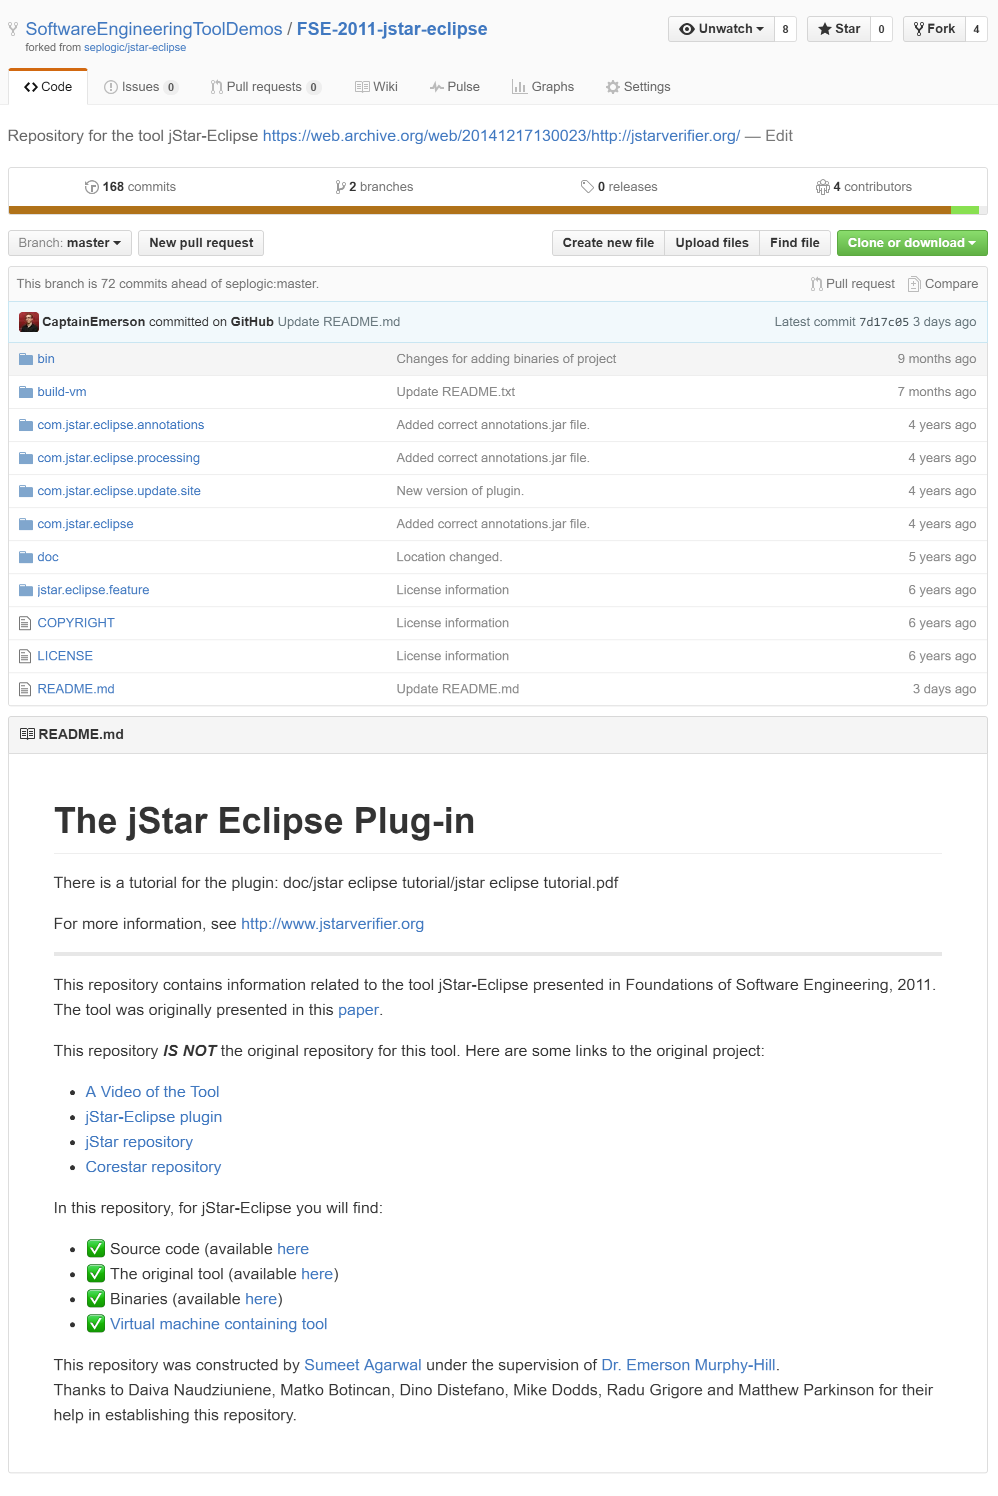
\includegraphics[width=0.5\textwidth]{jstar.png}
  \caption{Our forked repository for a jStar-eclipse.}\label{fig:jstar}
\end{figure}

Figure~\ref{fig:vagrant} shows the Vagrant script and 
part of an external script that builds the virtual machine.
The Vagrant script installs a plugin, 
uses a base virtual machine image from the boxcutter 
community,\footnote{\url{https://atlas.hashicorp.com/boxcutter}}
and calls four shell scripts interspersed with operating system 
restarts.
The external shell script shown removes some unneeded software,
and installs some prerequisites to the tool, including Eclipse and
an OCaml compiler. 

\begin{figure}[t]
  \centering
    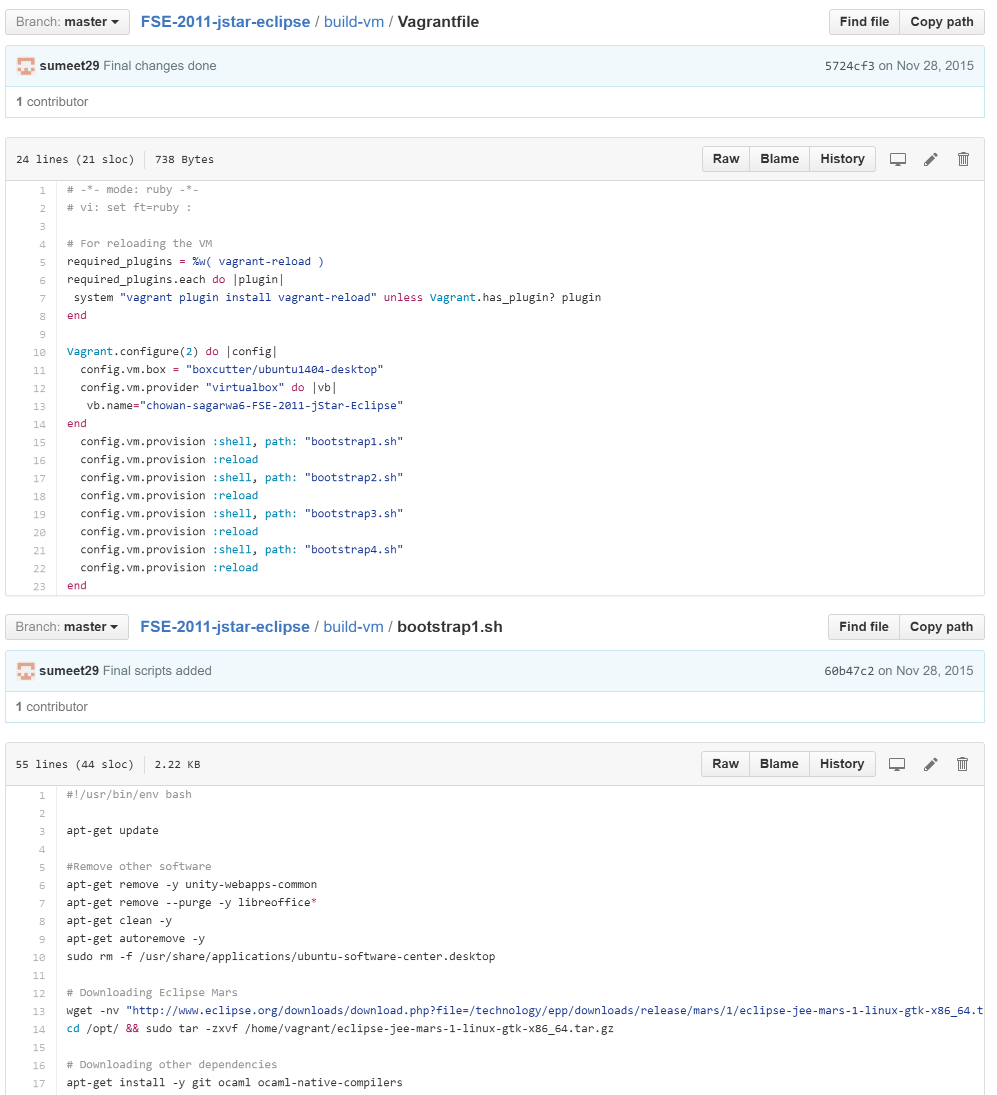
\includegraphics[width=0.5\textwidth]{vagrant.png}
  \caption{Scripts for generating virtual machine image containing jStar-eclipse.}\label{fig:vagrant}
\end{figure}

Figure~\ref{fig:vm} shows our virtual machine running 
jStar Eclipse.
In the figure, 
Eclipse has example code loaded that demonstrates
the tool, 
the tool plugin is installed into Eclipse,
Eclipse is installed on Ubuntu Linux,
and Ubuntu is running in a virtual machine
running Windows 10. 
In short, the user is relieved of having to install
the technology stack to run the tool; instead, 
she only has to download the virtual machine image.

\begin{figure}[t]
  \centering
    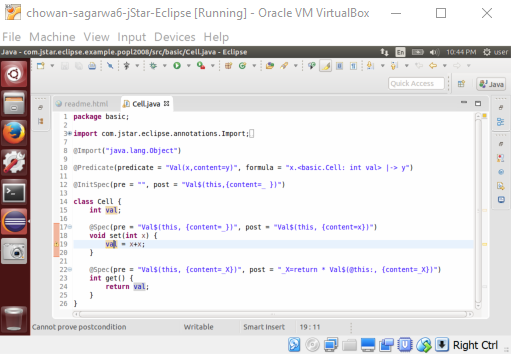
\includegraphics[width=0.5\textwidth]{vm.png}
  \caption{Screenshot of jStar Eclipse in a virtual machine.}\label{fig:vm}
\end{figure}

In the remainder of the paper, we do not call out 
any particular tool, but instead only speak of aggregates.
The reason is that we do not wish to embarrass any of the researchers.
Accordingly, we have taken steps to make sure that data we have made 
public with this paper does not embarrass researchers either.
For instance, while our GitHub repositories say when tools are 
not available, we do not publicly indicate why they are
not available.

\section{Results}

\subsection{RQ1: Effort to Get Tools Working}

Through a survey near the end of the course, 
teams estimated how long they spent
corresponding with researchers,
getting a tool to work,
getting it to work in a virtual machine,
and getting it to work with Vagrant.
Figure~\ref{fig:duration} shows the distribution of
these times in the form of a violin plot.
The median time teams spent corresponding with
researchers was \durationCorresponding hours.
For tools where teams obtained the tool,
they spent a median of \durationWorking hours
trying to get it to work.
For tools where the teams got a tool working,
they spent a median of \durationVM hours getting it working 
in a virtual machine image and
\durationVagrant hours generating a working tool
image with Vagrant.
In total, teams spent \durationTotal hours working
on all tools combined.

\begin{figure}[!ht]
  \centering
    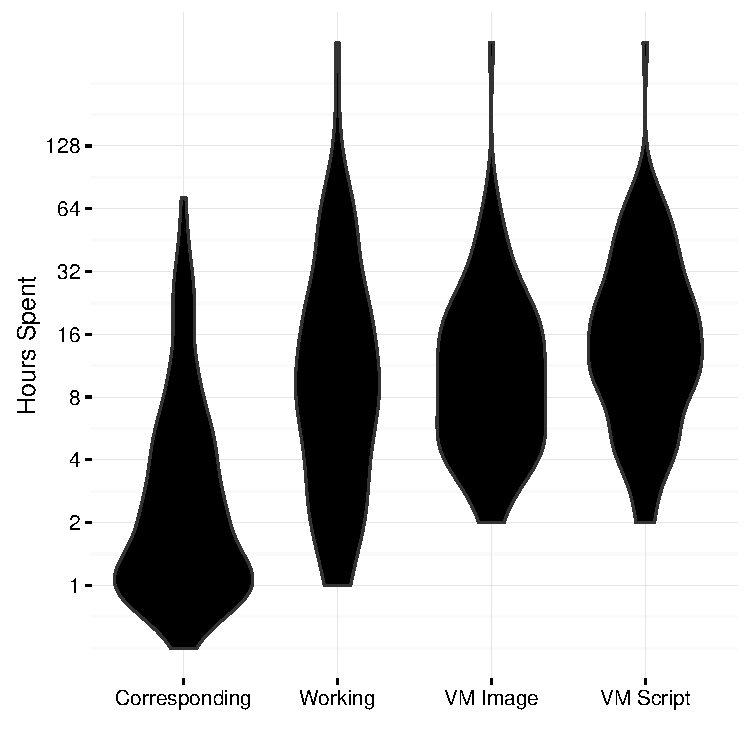
\includegraphics[width=0.5\textwidth]{durations.pdf}
  \caption{Time spent by teams performing four project activities.}\label{fig:duration}
\end{figure}

The survey also asked teams if they spent
time on other activities during the project.
In addition to project requirements like establishing
the GitHub repository, teams 
reported spending additional time 
learning about their tools,
searching for the tool on the web,
waiting for researcher replies,
obtaining the license for a tool,
figuring out what dependencies a tool had,
obtaining a Solaris base box for Vagrant,
and
getting a tool to work with a variety of examples.

\begin{figure}[!ht]
  \centering
    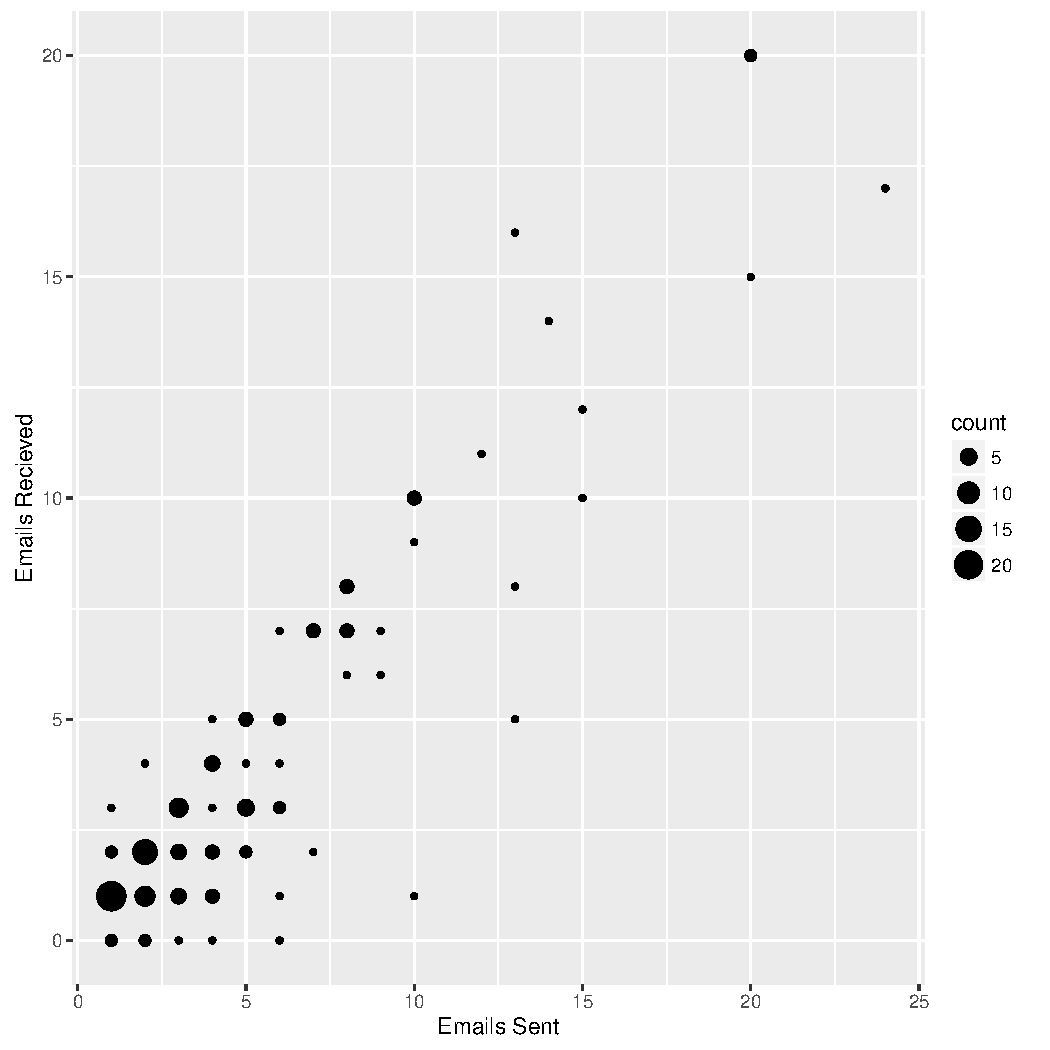
\includegraphics[width=0.5\textwidth]{emailPlot.pdf}
  \caption{Summary of emails sent and received.}\label{fig:emailSnR}
\end{figure}

Because a significant portion of teams' time was
spent corresponding with the researchers,
the survey also asked teams about their email interactions.
Overall, teams sent emails for \emailsPercentSent of tools.
Teams sent a median of \emailsSent and received 
a median of \emailsRecieved emails from each researcher.
Figure~\ref{fig:emailSnR} summarizes the number of emails
we sent and received, where the size of each dot
represents the number of tools that had
that many emails sent and received.
We see that, overall, few emails were required
and researchers appeared generally responsive.

The effort spent to get a tool working was not only
borne by us, but also the researchers who 
responded to our emails.
To minimize researchers' effort, we did not ask researchers directly.
Instead, we asked teams to estimate how much time researchers spent 
reading and responding to our emails, including time for 
any background work such as restarting servers.
Teams estimated that a median of \durationAuthorResponse minutes 
was spent, with \durationAuthorResponseCountHigh researchers having
to spend more than an hour.

\subsection{RQ2: Barriers to Getting Tools Working}

We next describe three barriers we encountered 
to getting the tools working:
obtaining the tools from the paper,
obtaining compliance from the researchers,
and technical challenges. 

%TODO numbers or percentages?

\subsubsection{Obtaining the Tools from the Paper}

Teams found that about \papersWithLinks papers
contained links to online information about their tools.
Teams also found that \papersWithLinksDead papers
had links that were no longer functional,
where \papersWithLinksRevived of those links
being fixed after teams emailed the researchers.

When it came to obtaining the tools, 42\%
could be obtained from links in 
the papers directly.
\obtainGoogle could not be obtained from
links in the papers themselves, but could be
from searching the web.
When those failed, another \obtainEmail were 
obtained after emailing the researchers.
In doing so, \contactFixLink links to tools 
were fixed by the tools' researchers.
\obtainNot of tools could not be obtained
by teams at all.

We also assessed where the source code for tools are available,
apart from our GitHub repositories.
\onlineNotAvail of tools had no source code available 
online.
\onlinePersonalSite of tools had source code hosted
on a researcher's personal website.
Many tools were available on open code repositories:
\onlineGitHub on GitHub, 
\onlineGcode on Google Code,
\onlineSourceforge on Sourceforge,
\onlineBitbucket on Bitbucket,
and \onlineCodeplex on CodePlex.
Of these, researchers began hosting \contactHosted tools 
on public repositories after
we contacted them.

Even when tools were ostensibly available,
sometimes critical pieces were missing,
as reported by teams in freeform text on the survey.
Teams reported missing configuration files,
settings that needed to be edited, 
information about IDE compatibility,
sample input,
and steps required for installation. 

\subsubsection{Researcher Compliance}

While researchers were generally responsive to emails,
they were not necessarily responsive or compliant 
with the requests contained in those emails.
Figure~\ref{fig:requests} lists what teams requested from researchers
(horizontally) and whether researchers complied (bars).
Overall, each kind of request was met with substantial non-response and
non-compliance.
Beyond these requests, teams reported needing to ask for 
license keys and
an old version of a dependency.

For \unworkNoResponseToAsk tools, teams reported asking for a tool,
but receiving no response from the researchers.
For \unworkTooLate tools, teams eventually got a response with the tool, 
but it was  too late (more than 7 days after initial contact).
\unworkInternal tools were not available outside the organization
they were developed in.
\unworkPay tools had software dependencies on for-pay tools; 
they may have worked if we had been willing to pay 
for the dependencies.

Several tools were not available, 
and the researchers were unwilling or unable make them so:
researchers for two tools were simply unavailable,
without further explanation; 
one researcher was uncomfortable making the tool available;
one said the tool was only a prototype;
one stated that the tool had too many dependencies with other tools;
and one stated that the tool does not exist anymore.

\begin{figure}[!t]
  \centering
    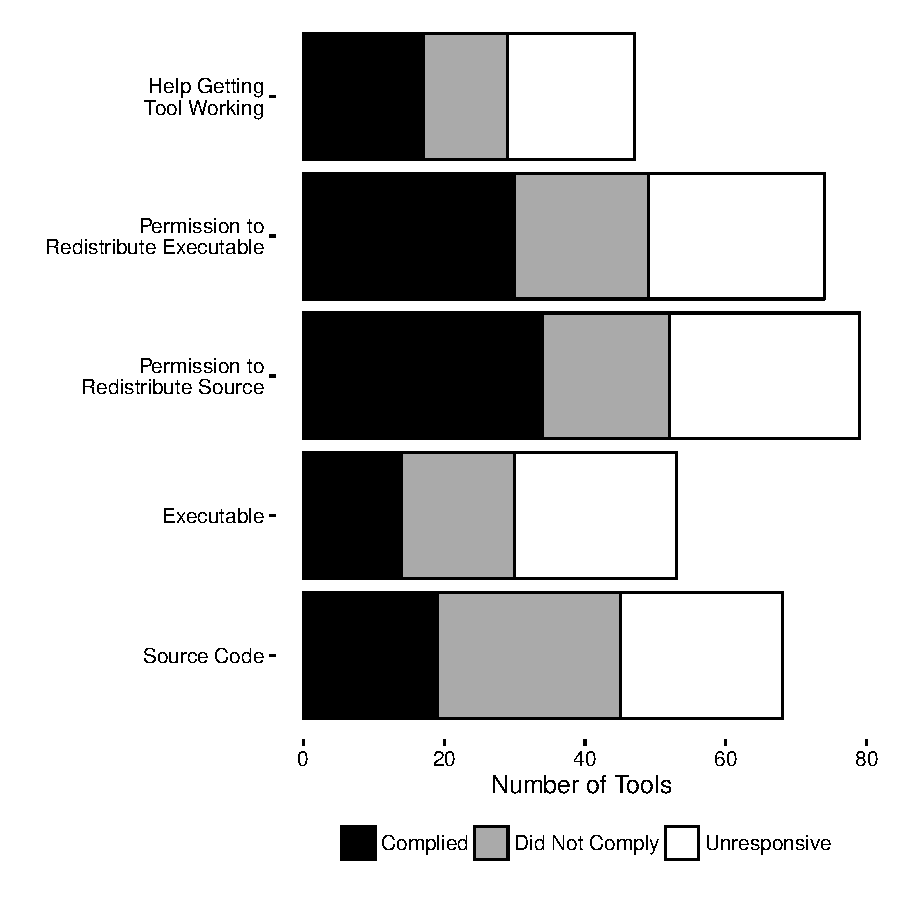
\includegraphics[width=0.5\textwidth]{requestPlot.pdf}
  \caption{Researchers compliance with teams' tool requests.}\label{fig:requests}
\end{figure}

%TODO should check to see which projects have licenses, 
%and perhaps students didn't need to send emails

Teams also reported about the tone of the response they received from 
researchers.
Teams felt that \emailsHelpful of responses were helpful and
\emailsFriendly were friendly.
Only \emailsIntimidating felt the responses were intimidating
and \emailsAnnoyed seemed annoyed.                                                                                                              


\subsubsection{Technical Challenges}

In total, teams marked \working tools as working.
The remaining tools were marked ``unworkable'' for a 
several of reasons.
The most common reason teams marked tools as unworkable
was that the teams could not get the tools 
working (\unworkCouldntWorkIt tools),
typically due to build errors or mismatches between
the way the downloaded tool worked and the way 
it was described in the paper.
A common problem for these tools was dependencies on
software whose versions were unspecified 
(and at least once forgotten by the researcher), and teams
failed to get the tools working with the versions they
tried.
Teams described problems with 
tool configuration,
missing functionality, and
missing or corrupted program files or data.
After contacting the researchers, teams reported that researchers 
fixed bugs in \contactFixBug tools,
fixed deployment issues in \contactFixDepl tools,
and fixed some problems with dependencies in one tool.

\subsection{RQ3: Barriers to Virtualizing}

Once the tools were available and working, 
the barriers to getting them working in the
virtual machines were largely about licensing issues
surrounding each tool and the software it depends on.

\redistPermissionArtifact tools were open-sourced, 
under a variety of licenses, making them appropriate
for redistribution in virtual machines.
Common licenses were:
\licenseEPL with an Eclipse Public License license,
\licenseMIT with an MIT license,
\licenseApache with an Apache 2.0 license,
\licenseBSD with a BSD 2.0 license,
\licenseGPL with a GPL 2.0 license,
\licenseGPLThree with a GPL 3.0 license,
\licenseLGPL with a LGPL 2.0 license,
\licenseMPL with a Microsoft Public License.
Researchers added open source licenses to \contactOSSed tools
after we contacted them by email.	
Although they did not have an explicit license,
researchers of \redistPermissionEmail tools granted us
permission to redistribute via email.
Two tools were freely available online
with an open source license, but the researchers
specifically asked us \emph{not} to redistribute the
tool; although we honored the researchers' requests,
the requests nonetheless directly conflicts
with those tools' licenses.  

Our ability to redistribute virtual machines of the tools were
further restricted by the tools' dependencies.
The most common dependencies were on the Windows 
operating system (\depWindows tools).
\depVS tools were dependent on Visual Studio.
A few other tools depended on other commercial 
operating systems and tools.
 
After excluding tools 
that we did not get working,
that we did not have permission to redistribute, and 
that relied on software we did not have permission to redistribute,
\permissionToRedistribute tools remained.
We have made these tools publicly available in virtual machines 
images online.\footnote{\url{http://go.ncsu.edu/SE-tool-VMs}}
Our GitHub repositories link to these virtual machine images,
and contain relevant tool artifacts such as source code
and binaries.
A total of 62 repositories 
% based on https://github.com/search?q=org%3ASoftwareEngineeringToolDemos+Vagrant.configure&ref=searchresults&type=Code&utf8=%E2%9C%93
contain Vagrant scripts to build 
virtual machines that contain the tools. 

\subsection{RQ4: Classroom}

In the context of a university course,
students viewed the course project negatively,
based on two main metrics.
First, many students dropped the course; 
at its peak, the course was full and had a full
waiting list with a combined 105 students.
By the end of the course, only 58 students remained.
%based on mypack, minus one student marked as `Crs Wdraw'
Second, the university-administered evaluations for
the course and course project were low.
All quantitative metrics for the course were below
the Computer Science department average, and were
lower than for courses the instructor has previously
taught.
Specifically, the most common response to the question
of whether the course project was a valuable aid to learning
was ``strongly disagree''.
What accounts for this negative reaction?

With respect to students dropping the course, students were asked
in the non-anonymous survey at the end of the course whether they knew
students who dropped, and if so, whether they knew why.
While students cited some external reasons, the 
primary one appeared to be that the course was more work
than they had expected.
Although other changes had been made to the course, 
of which ``flipping'' the lectures~\cite{flipped} is worth mentioning,
the main change was the semester long project. So the project workload
was likely responsible for the drops.

With respect to low student evaluations of the project,
the problem appears to be with several aspects of project
design, rather than a fundamental issue with the project itself.
In the non-anonymous survey, students were given a brief description
of the old project, and were asked which version of the course project
they would prefer.
\projectLikeThis of students preferred the present course project,
\projectLikeOther would prefer the past course project,
and the remaining students had no preference.
Nonetheless, several areas of the course project were challenging,
as described below.

\textbf{Lack of Teamwork.}
  	Teamwork was critical to a successful project, because a single student
  	is unlikely to have all the technical skills necessary to get an
  	arbitrary tool working.
  	While the instructor explained this to students early on, 
  	he did not provide an environment that was conducive to teamwork.
  	First, no specific collaboration technologies or practices were encouraged,
  	such as Slack, scrum, or cloud-based virtual machines.
  	Second, the easiest way to break down work was to assign one person in a team
  	to work on one tool; because each tool generally worked independently
  	from other tools, it appeared that teammates worked in a siloed way.  	
  	Third, teams lacked cohesiveness because teammates were assigned randomly.
  	Because many students dropped the course, team cohesiveness may have 
	been reduced further.
	Teamwork problems can likely be improved substantially in the future by 
	educating students on and providing collaboration technologies, and allowing
	teams to choose their own members. 

\textbf{Uneven Tool Difficulties.}
  	Some tools are simple, others are complex; likewise,
  	some tools were easy to get working, while others were extremely difficult.
  	The instructor originally aimed to improve fairness by assigning multiple tools
  	to teams, so that average tool difficulty across teams should be roughly equivalent.
  	However, intra-team siloing resulted in some students doing
  	significantly more work than other students. 
  	Moreover, it was difficult for teams to estimate the difficulty of a 
  	tool from the paper alone.
  	Breaking down the silos may improve this inequity problem.
  	This may also be an opportunity to create an assignment that applies the course
  	material on effort and risk estimation.   	

\textbf{Vagrant Scripting.}
  	Vagrant scripting turned out more challenging than anticipated.
  	One reason was that installing software on Windows machines is difficult
  	due to operating system security checks.
  	Another difficulty was some scripts needed large files, which GitHub could not
  	store, so these scripts needed to load data from other locations 
  	(such as Google Drive), decreasing our repositories' archival value. 
  	Building Vagrant scripts should be easier in the future, now that
  	we have a repository of examples that include, for instance, how to
  	use a Windows package manager and how to 
  	install Eclipse and load Eclipse workspaces. 
  	One way to approach quality problems is by treating them as testing and 
  	continuous integration problems; Travis CI,
  	for instance, may be appropriate for building VMs automatically,
  	assessing the quality of those VMs with test automation,
  	and making public the VMs and Travis scripts.

\textbf{Unusual Grading.} 
	The instructor recognized that the grading strategy of making substantial
	grade adjustments when teams got unworkable tools working would be 
	controversial.
	Four out of 44 students complained about this in the anonymous course
	evaluation.
	Only one team ended up getting an unworkable tool working, and this team expressed
	some hesitation in doing so because it meant negative repercussions for their
	classmates.
	Nonetheless, in the opinion of the instructor, the grading strategy was effective
	in making sure teams tried sufficiently hard to get their tools working. 
 	Future iterations of the project may explore alternate grading options.

\textbf{In-Class Presentations.}
  	Although in-class presentations were only 5 minutes per tool, as a whole they
  	took up an inordinate amount of class time.
  	For future iterations of the projects, all students will instead make videos 
  	about their tools, and perhaps only one tool per team will be presented
  	in class.
  	%pmchen3: DE students were required to make a video, or is this more focused on the in-class portion?
  	%CaptainEmerson: they did make a video; clarified ``all'' here
 
\vspace{3mm}
Finally, despite the challenges with the course, the instructor's opinion is that 
the course was highly worthwhile.
He knows of no other software engineering courses that integrate research into 
teaching to the degree that this one does, while at the same time capitalizing
on the existing talents of computer science graduate students for the greater 
good.
While educational outcomes can be strengthened by deeper integration of the lecture
material into project work, as a whole, the instructor believes that 
the project was an improvement over the prior project.
On the other hand, the project was so radically different from prior 
projects -- perhaps to a mutinous degree -- that trying it is a risky 
proposition for untenured instructors.

\section{Discussion}

* Email is soooo bad; non-response vs. non-compliance. lots of requests just ``got lost''
* Should AECs use Vagrant scripts? Good for archival purposes. Sidestepped Windows licensing issues.
* Have we really solved the bitrot problem? Do VMs bitrot?
* Consider problem of Topaz (?), system that maybe had circular menus; but what did they look like, and what were they for.
* Arguably as SE researchers we should be the best!
* What should we require for demos?
* How does this extend to main track papers?

\subsection{On Software Licensing}

At several points during the project, software licensing posed significant
problems for redistributing tools.

First, we were surprised that several researchers asked us not to redistribute
their tools, even though those tools' licenses explicitly allowed for redistribution.
They provided essentially two rationales for this.
One was that, although they initially chose an open source license, 
their university's tech transfer office later advised them not to make the source code available.
The other was that they did not want potential tool users to become confused 
because the source code was stored in two places (in their repository, and in ours).
It seems that these authors did not really want an open source license
in the first place; perhaps instead they should have given their software
no license at all or simply asserted copyright over it.

Second, several researchers provided us explicit permission to redistribute their tools,
but without an explicit open source license, this raises a number of questions.
Can a third party who downloads our virtual machine with the researchers' tool use the tool for any purpose?
Can a third party redistribute the tool?
If so, how is that third party supposed to know about our private communication?
These questions underscore the need for researchers to explicitly license their tools
when they are released.

Third, dependencies on commercial software, such as Microsoft Windows, made it
impossible for us to redistribute virtual machines.
However, Vagrant provided a nice solution to this problem, since Vagrant scripts
use

\subsection{Tools as Unreachable Services}

Several of the tools we analyzed were a service or had a
service component; for instance, several tools
ran as web applications on the creator's website.
In total, for \serviceRunning tools, teams 
reported that the service was running when the teams tried
to access it.
For \serviceRunningLater tools, teams reported that the service
was not running, but the researchers got the service running
after the teams emailed them.
For \serviceRunningNever tools, teams reported that the service
never worked when they tried it. 

While services may excel in convenience to the user, 
they can do so only if they are running.
In a sense, non-working services are worse than non-working source code;
at least with source code, a user who wants to try the tool can 
at least modify the code and resolve dependencies manually.
With a tool as a service, the user's success is entirely dictated
by the researcher, who, as our observations suggest, is often
unresponsive or noncompliant. 
Thus, we cannot recommend services as  way for software
engineering researchers to release their tools,
at least without also making the underlying software for 
the service available as well.  

\subsection{Tools Do Not Keep Well}

This study illustrates some interesting points about how well tools
are archived for posterity, even those in those from only a few years ago.
Two tools illustrated archiving failure.
One researcher told us the tool was simply no longer available.
Another researcher told us that the tool's server crashed and they
would need to locate the tool on a backup; that researcher never got back to us.
But these only illustrate explicit failures -- there may be others 
that we were unable to observe.
For instance, perhaps ``the tool was just a prototype'' is a euphamism for 
``we don't know where it is.''
And the researchers who did not respond to our emails 
could have lost their tools as well.

We also encountered systematic near-failures of tool archives.
Specifically, \onlineJustGcode of tools were hosted on Google Code
and no where else.
Because Google is retiring the hosting site, after 2016,
they no longer guarantee that these tools will be available.
Thus, if we hadn't cloned these tools' history to our repositories,
they may have been lost forever.
And even then, there are no guarantees

These observations underscore need for long-term archiving of research
tools becaues the current archival practices are failing.
 
\subsection{Threats to Validity}

%Generalizability to other projects, students=researchers?

Finally, threat to this research is the quality
of the resulting software; 	
having more than 60 capable 
graduate students repackaging tools enabled this study 
to scale up far beyond what a small research group could 
do, the disadvantage is a reduction of quality control.
We attempted to increase software reliability by
instituting peer evaluations, teacher's assistant evaluations,
and spot checks by the instructor for the artifacts produced
as part of this study.
Nonetheless, some quality problems likely occurred in our study.
For instance, consider Krishnamurthi's partial replication of 
Collberg and Proebsting's tool buildability study~\cite{collberg2016repeatability},
which disputed the buildability of several tools~\cite{skRep}.
Despite the software quality threat, there is a silver lining
to our study; because we have asked for and have exercised 
permission to redistribute virtual machines and Vagrant scripts,
any software quality problems that are found later can be 
corrected.
In fact, in future iterations of the course, the instructor 
plans on familiarizing students with the requisite technology
by finding and fixing bugs in GitHub repositories and 
Vagrant scripts via pull requests.

Similarly, data quality is a threat that arises from the large
number of participants on this project.
Some of the data presented in this paper highlights this threat.
For instance, there are three long tails in the violin plots in 
Figure~\ref{fig:duration}; these are caused by a single person 
filling in the maximum allowed value in the tool survey.
However, these outliers are likely inaccurate representations
of the actual amount of work performed.
The first author attempted to address such outliers by following
up with participants who reported them, but some participants 
were unresponsive.
Because we are uncertain of the veracity of such outliers,
we include them nonetheless.

\section{Conclusions}

Some other things.
We're critical of current practices, but we're just as guilty.
We'll have to solve this altogether.

% Something stating how many students opted to take part in the 
% paper? Does this show any worth as far as credibility and 
% success of the project?

\section*{Acknowledgments}

Thanks to Tim Menzies, Gail Murphy, and Thomas Zimmermann
for their helpful comments on drafts of this paper.  

\bibliographystyle{abbrv}
\bibliography{references} 

\end{document}
